\section{匀变速直线运动的推论}
\subsection{平均速度}
平均速度的定义为:
$$\overline{v}=\cfrac{x}{t}$$
将匀变速直线运动的位移\eqref{eq:displacement}式代入平均速度公式可得:
\begin{equation}
\overline{v}=\cfrac{v+v_0}{2}
  \label{eq:average}
\end{equation}

\subsection{中间时刻的瞬时速度}

记中间时刻的瞬时速度为$v_{\frac{t}{2}}$,则由匀变速直线运动速度与时间的关系\eqref{eq:v-t}得:
\begin{align}
v_{\frac{t}{2}}-v_0 &=a\cfrac{t}{2}\\
v-v_{\frac{t}{2}} &=a\cfrac{t}{2}
\end{align}
显然上面二式的右侧相等,所以有
\begin{equation*}
v_{\frac{t}{2}}-v_0=v-v_{\frac{t}{2}}
\end{equation*}
解得:
\begin{equation}
v_{\frac{t}{2}}=\cfrac{(v+v_0)}{2}
  \label{eq:v-half-t}
\end{equation}
对比平均速度公式,此二式可以合写成:
\begin{equation}
\overline{v}=v_{\frac{t}{2}}=\cfrac{(v+v_0)}{2}
  \label{eq:v-average-half}
\end{equation}

\subsection{位移中点的瞬时速度}

位移中点的瞬时速度记为$v_{\frac{x}{2}}$,由匀变速直线运动位移与速度\eqref{eq:x-v}式可得:
\begin{align}
v^2-v_{\frac{x}{2}}^2 &=2a\cfrac{x}{2}\\
v_{\frac{x}{2}}^2-v_0^2 &=2a\cfrac{x}{2}
\end{align}
显然上面二式的右侧相等,所以有
\begin{equation*}
v^2-v_{\frac{x}{2}}^2=v_{\frac{x}{2}}^2-v_0^2
\end{equation*}
解得:
\begin{equation}
v_{\frac{x}{2}}=\sqrt{\cfrac{v^2+v_0^2}{2}}
  \label{eq:v-half-x}
\end{equation}

\subsection{$v_{\frac{t}{2}}$和$v_{\frac{x}{2}}$的大小关系}

\subsubsection{从物理角度证明}

如图\ref{fig:+t-x-middle} 画出了\CJKunderwave{匀加速直线运动}时间中点和位移中点的具体位置.

\begin{figure}[H]
  \centering
  \begin{tikzpicture}
    \draw (0,0) node [anchor=north east]{0}--(4,0) node [anchor=north west]{x};
    \draw (0,0) -- (0,0.25);
    \draw (4,0) -- (4,0.25);
    \draw (1,0) -- (1,0.25) node [anchor=south]{$v_{\frac{t}{2}}$};
    \draw (2,0) -- (2,0.25) node [anchor=south]{$v_{\frac{x}{2}}$};
    \draw (1,0) node [anchor=north]{A};
    \draw (2,0) node [anchor=north]{B};
  \end{tikzpicture}
  \caption{匀加速直线运动}
  \label{fig:+t-x-middle}
\end{figure}

由于图\ref{fig:+t-x-middle} 所示为匀加速直线运动,所以质点从A点到B 点必须\CJKunderwave{加速一段时间},所以可以得到时间中点的瞬时速度 $v_{\frac{t}{2}}$ 小于位移中点的瞬时速度 $v_{\frac{x}{2}}$

如图\ref{fig:-t-x-middle} 画出了\CJKunderwave{匀减速直线运动}时间中点和位移中点的具体位置.

\begin{figure}[H]
  \centering
  \begin{tikzpicture}
    \draw (0,0) node [anchor=north east]{0}--(4,0) node [anchor=north west]{x};
    \draw (0,0) -- (0,0.25);
    \draw (4,0) -- (4,0.25);
    \draw (3,0) -- (3,0.25) node [anchor=south]{$v_{\frac{t}{2}}$};
    \draw (2,0) -- (2,0.25) node [anchor=south]{$v_{\frac{x}{2}}$};
    \draw (2,0) node [anchor=north]{A};
    \draw (3,0) node [anchor=north]{B};
  \end{tikzpicture}
  \caption{匀减速直线运动}
  \label{fig:-t-x-middle}
\end{figure}

由于图\ref{fig:-t-x-middle} 所示为匀减速直线运动,所以质点从A点到B 点必须\CJKunderwave{减速一段时间},所以仍然可以得到时间中点的瞬时速度 $v_{\frac{t}{2}}$ 小于位移中点的瞬时速度 $v_{\frac{x}{2}}$

综合以上论述可得:

\begin{equation}
  v_{\frac{t}{2}} < v_{\frac{x}{2}} 
  \label{eq:v-t<x}
\end{equation}

\subsubsection{从数学角度证明}

对于任意的 $a>0$ ,$b>0$ 有下述均值不等式:
\[
  \sqrt{\cfrac{a^2+b^2}{2}}\geqslant\cfrac{a+b}{2}
\]

上式中,当且仅当 $a=b$ 取等号.为了保证同学们学习的连惯性,这里证明此式如下:

\begin{gather*}
 (a-b)^2 \geqslant 0\\
 a^2+b^2 -2ab \geqslant 0\\
 a^2+b^2 \geqslant 2ab
\end{gather*}

对上式,左右同时加上 $a^2+b^2$ 得

\[
2(a^2+b^2) \geqslant a^2+b^2+2ab
\]

上式右侧为完全平方式,将其写成完全平方式

\[
2(a^2+b^2) \geqslant (a+b)^2
\]

左右同时除以$4$ ,再开方,得

\[
  \sqrt{\cfrac{a^2+b^2}{2}}\geqslant\cfrac{a+b}{2}
\]

无论是匀加速还是匀减速,都有$ v\neq v_0$,如设运动的方向为正,则二个速度都大于零.所以有
\[
  \sqrt{\cfrac{v^2+v_0^2}{2}}
  >
  \cfrac{v+v_0}{2}
\]

上面正是时间中点的瞬时速度和位移中点的瞬时速度的表达式,所以有

\begin{equation*}
  v_{\frac{t}{2}} < v_{\frac{x}{2}} 
\end{equation*}

\subsection{相邻相等时间段内的位移差}
设匀变速直线运动的加速度为$a$,任意相邻二段时间为$T$,此二段时间内的位移分别为$x_1$ 和$x_2$,如图\ref{fig:Delta x} 所示
\begin{figure}[H]
  \centering
  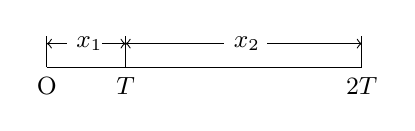
\begin{tikzpicture}
    \draw (0,0)--(4,0);
    \draw (0,0) node [anchor=north]{\small O}--(0,0.4);
    \draw (1,0) node [anchor=north]{\small $T$}--(1,0.4);
    \draw (4,0) node [anchor=north]{\small $2T$}--(4,0.4);
    \draw [<-](0,0.3)--(0.25,0.3) node [anchor=west]{\small $x_1$};
    \draw [->](0.7,0.3)--(1,0.3);
    \draw [<-](1,0.3)--(2.25,0.3) node [anchor=west]{\small $x_2$};
    \draw [->](2.8,0.3)--(4,0.3);
  \end{tikzpicture}
  \caption{等时间段内的位移差}
  \label{fig:Delta x}
\end{figure}

则有关系
\begin{equation}
x_2-x_1=aT^2
  \label{eq:Delta x}
\end{equation}
式\eqref{eq:Delta x} 不涉及初速度,一般用来处理用打点计时器所获得的纸带,因为纸带上的点是可以用毫米刻度尺来测量的,用这个方法求加速度很方便.

\subsubsection{证法一}
第一段中间时刻的瞬时速度等于第一段的平均速度,记为$v_1$,则$v_1=\cfrac{x_1}{T}$
第二段中间时刻的瞬时速度等于第二段的平均速度,记为$v_2$,则$v_2=\cfrac{x_2}{T}$
由\eqref{eq:acceleration}式得
$$a=\cfrac{v_2-v_1}{T}$$
将$v_1$和$v_2$的表达式代入得
$$a=\cfrac{x_2/T-x_1/T}{T}$$
上式分子分母同乘以$T$,然后左右同时再乘以$T^2$,移项得
$$x_2-x_1=aT^2$$
\subsubsection{证法二}
画出这段时间段内的$v-t$图象如下
\begin{figure}[H]
  \centering
  \begin{tikzpicture}
    \draw[->] (0,0) node [anchor=north]{O} -- (3.5,0) node [anchor=north]{t};
    \draw[->] (0,0)  -- (0,2.5) node [anchor=west]{v};
    \draw (0,0.5) -- (3.4,2.2);
    \draw [dotted] (1.5,0) node [anchor=north]{T}-- (1.5,1.25);
    \draw  (3,0) node [anchor=north]{2T} -- (3,2);
    \draw [dotted] (0,0.5)--(3,0.5);
    \draw [dotted] (1.5,1.25)--(3,1.25);
    \draw [pattern=north west lines] (0,0)--(1.5,0)--(1.5,1.25)--(0,0.5);
    \draw [pattern=north west lines] (1.5,1.25)--(3,1.25)--(3,2);
    \draw [pattern=north west lines] (1.5,0) rectangle (3,0.5);
    \draw (3,0.875) node [anchor=east] {\small $x_2-x_1$}; 
    \draw (0,0.5) node [anchor=east]{\small $v_0$};
    \draw [dotted] (0,1.25) node [anchor=east]{\small $v_0+aT$}--(1.5,1.25);
  \end{tikzpicture}
  \caption{相邻位移差}
  \label{fig:Delta xx}
\end{figure}

图\ref{fig:Delta xx} 中$0\sim T$ 时间段内梯形阴影面积表示位移$x_1$,$T\sim 2T$ 梯形面积表示位移$x_2$ 两面积之差就表示$x_2-x_1$,在图中所示为空白矩形的面积.矩形的长为$T$,宽为$aT$,所以其面积为$aT^2$,即
$$x_2-x_1=aT^2$$

\subsubsection{证法三}
设初速度为$v_0$,则由匀变速直线运动位移与时间的关系\eqref{eq:x-t}得
\begin{equation}
x_1=v_0T+\cfrac{1}{2}aT^2
  \label{eq:x1}
\end{equation}
\begin{equation}
x_1+x_2=v_0\cdot 2T+\cfrac{1}{2}a(2T)^2
  \label{eq:x2+x1}
\end{equation}
用式\eqref{eq:x2+x1}$-2\times$\eqref{eq:x1}得
$$x_2-x_1=aT^2$$

\subsubsection{证法四}
同证法三计算出第一段的位移,即式\eqref{eq:x1}.由匀变速直线运动速度与时间的关系\eqref{eq:v-t}得第二段的初速度为

$$v_1=v_0+aT$$

再由匀变速直线运动位移与时间关系\eqref{eq:x-t}计算第二段的位移得

\begin{equation}
x_2=(v_0+aT)\cdot T+\cfrac{1}{2}aT^2
  \label{eq:x2}
\end{equation}

用式\eqref{eq:x2} $-$ \eqref{eq:x1}得
$$x_2-x_1=aT^2$$

\subsection{逐差法求加速度}
在用打点计时器处理纸带时得到以下数据,为了说理清析,仅以图\ref{fig:zhidai} 为例说明处理的原理.
\begin{figure}[H]
  \centering
  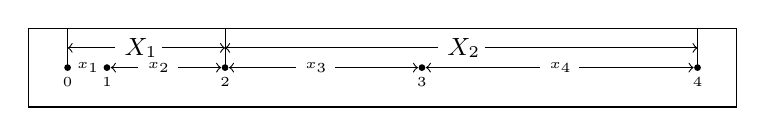
\begin{tikzpicture}
    \foreach \x in {0,0.5,2,4.5,8}
    \draw [fill=black](\x,0) circle (1pt); 
    \draw (-0.5,-0.5) rectangle (8.5,0.5);
    \draw (0,0) node [anchor=north]{\tiny 0};
    \draw (0.5,0) node [anchor=north]{\tiny 1};
    \draw (2,0) node [anchor=north]{\tiny 2};
    \draw (4.5,0) node [anchor=north]{\tiny 3};
    \draw (8,0) node [anchor=north]{\tiny 4};
    \draw (0,0) node [anchor=west] {\tiny $x_1$};
    \draw [<-] (0.55,0) -- (0.9,0) node [anchor=west] {\tiny $x_2$};
    \draw [->] (1.4,0) -- (1.95,0);
    \draw [<-] (2.05,0) -- (2.9,0) node [anchor=west] {\tiny $x_3$};
    \draw [->] (3.4,0) -- (4.45,0);
    \draw [<-] (4.55,0) -- (6,0) node [anchor=west] {\tiny $x_4$};
    \draw [->] (6.5,0) -- (7.95,0);
    \foreach \x in {0,2,8}
    \draw  (\x,0)--(\x,0.5);
    \draw [<-](0,0.25)--(0.6,0.25) node [anchor=west]{\small $X_1$};
    \draw [->](1.2,0.25)--(2,0.25);
    \draw [<-](2,0.25)--(4.7,0.25) node [anchor=west]{\small $X_2$};
    \draw [->](5.3,0.25)--(8,0.25);
  \end{tikzpicture}
  \caption{逐差法四段纸带}
  \label{fig:zhidai}
\end{figure}

使用毫米刻度尺测量长度时,计数与真实值的差距不会大于$1mm$,这个$1mm$ 叫做绝对误差.无论这个真实长度是多大,这个绝对误差也不会发生变化,但是这个绝对误差在实际长度中占的比例却不相同,这个比例叫做相对误差,即
$$\mbox{相对误差}=\cfrac{\mbox{绝对误差}}{\mbox{实际长度}}\times 100\%$$
所以实际长度越长,相对误差越小,也就是在绝对误差一定($1mm$)的情况下,测量越长的长度相对误差越小.

在如图\ref{fig:zhidai} 所获得的纸带中,如果实际测量,则要求测量$0\rightarrow 1$,$0\rightarrow 2$,$0\rightarrow 3$,$0\rightarrow 4$ 的长度来标注的.但是在纸带上说理却一般如上图所示.

在使用\eqref{eq:Delta x} 来计算加速度时,显然所取长度越大则相对误差越小.在所示纸带中,能找到的长度最大的相邻位移就是图中的$X_1=x_1+x_2$ 和 $X_2=x_3+x_4$ ,但是此二大段的时间间隔却对应由原来的$T$ 变成了$2T$,对这二大段使用\eqref{eq:Delta x} 得
$$(x_3+x_4)-(x_1+x_2)=a(2T)^2$$
由上式解得
$$a=\cfrac{(x_3+x_4)-(x_1+x_2)}{(2T)^2}$$

同理,其它偶数段类似.如果纸带中有6段,对应分成两大组,每组的时间为$3T$,则对应的逐差法为
\begin{equation}
a=\cfrac{(x_4+x_5+x_6)-(x_1+x_2+x_3)}{(3T)^2}
  \label{eq:zhucha}
\end{equation}


如果{\heiti 一段纸带有奇数段},则处理思路上有点特别.我们来仔细审查一下这个求解过程.在使用$\Delta x =aT^2$ 时,我们需要计算这个$\Delta x$ ,而测量时这需要$3$个或$4$个测量值,设置第$0$个点为原点(注意,原点是测量时刻度尺上的$0$刻度对齐的,所以这个读数可以认为不存在误差),以$x$ 上加一个撇号表示该点的坐标,例如$x'_2$ 表示第$2$个点的坐标,比如前两段差
$$\Delta x_{12}=x_2-x_1=x'_2-x'_1-x'_1$$
纸带上\CJKunderwave{任何二段的差都需要四个坐标}来确定.然而实际读数时,读数误差为$1mm$,所以原则上任意二段位移差的最大绝对误差为$4mm$.例如我们求解加速度可以使用 
$$a_1=\frac{x'_2-x'_1-x'_1}{T^2}$$
也可以使用
$$a_2=\frac{(x'_3-x'_2)-(x'_2-x'_1)}{T^2}$$
考虑$a_1$和$a_2$的误差,则分母都是$T^2$,但是$a_1$分子上为三个坐标,因为原点是我们测量时对齐的,所以误差是$3mm$,但是$a_2$的中分子是四个坐标,所以它的误差为$4mm$所以$a_1$和$a_2$相比误差更小一些.但是如果我们取它们的几何平均值作为该质点运动的加速度,即
$$a_{12}=\frac{1}{2}(a_1+a_2)=\frac{x'_3-x'_2-x'_1}{2T^2}$$
此时仍然认为分母$T^2$则分子是$(x'_3-x'_2-x'_1)/2$,三个坐标的误差最大为$3mm$,所以以$a_{12}$作为所示加速度时误差为$1.5mm$.如果一段纸带有$7$段,则可以取
$$a_1=\frac{x_5'-x_4'-x_1'}{4T^2}$$
$$a_2=\frac{x_6'-x_5'-x_2'+x_1'}{4T^2}$$
$$a_3=\frac{x_7'-x_6'-x_3'+x_2'}{4T^2}$$
上述三式中,$a_1,a_2,a_3$的分子误差分别为$3mm/4=0.75mm$,$4mm/4=1mm$ ,$4mm/4=1mm$ 但是若取这三者的几何平均作为测量加速度,即
$$a=\frac{1}{3}(a_1+a_2+a_3)=\frac{x_7'-x_4'-x_3'}{12T^2}$$
上式中分子部分误差可以降到$3mm/12=0.25mm$,如果使用前$6$段,或者后$6$段来计算加速度,则同理可得前$6$段分子上的误差为$3mm/9\approx 0.33mm$ ,而后$6$段计算时,分子上的误差为$4mm/9\approx 0.44mm$,显然这几个误差相比较的话去掉中间一段时所得结果误差最小,能小到取相邻$6$段时误差的$75\%$!!所以在同学们计算加速度时要\CJKunderwave{去掉奇数段中间的一段},如下
$$a=\cfrac{(x_5+x_6+x_7)-(x_1+x_2+x_3)}{12T^2}$$

\subsection{初速度为零的比例关系}

匀变速直线运动的比例关系共有两大组,其一按\CJKunderwave{时间等分},其二按\CJKunderwave{位移等分}.

\subsubsection{按时间等分}

时间每隔 $T$ 分一份,则 $T$ ,$2T$,$3T$,$\cdots$ 等时刻对应的速度分别为 $v_1$,$v_2$,$v_3$,$\cdots$

由\eqref{eq:v-t} 式,可得
\[
  v_n=a\cdot nT
\]

所以有

\begin{equation}
  v_1 : v_2 :v_3 : \cdots : v_n = 1 : 2 : 3 :\cdots  : n 
  \label{eq:v-frac}
\end{equation}

从0时刻开始,$0\sim T$, $0\sim 2T$, $0\sim 3T $ ,$ \cdots$ 等时间间隔内对应的位移分别记为 $x_1$ , $x_2$ , $x_3$, $\cdots$

由 \eqref{eq:x-t} 式,可得

\[
  x_n=\cfrac{1}{2}a\cdot (nT)^2
\]

所以有

\begin{equation}
  x_1 : x_2 :x_3 : \cdots : x_n = 1^2 : 2^2 : 3^2 :\cdots  : n^2 
  \label{eq:x-frac}
\end{equation}

第 $T$ ,第 $2T$ ,第 $3T$ , $\cdots$ ,第 $nT$ 时间间隔内对应的位移分别记为
$\Delta x_1$ , $\Delta x_2$ , $\Delta x_3$, $\cdots$ , $\Delta x_n$

由$x_n$ 与 $n$ 的关系可得
\[
  \Delta x_n =x_n-x_{n-1}=(2n-1)\cdot \cfrac{1}{2}aT^2
\]

所以有

\begin{equation}
 \Delta x_1 :\Delta x_2 :\Delta x_3 : \cdots :\Delta x_n 
 = 1 : 3 : 5 :\cdots  : (2n-1)
  \label{eq:Delta x-frac}
\end{equation}

\subsubsection{按位移等分}

位移每隔$L$ 分一份,记 $L$ ,$2L$ , $3L$ , $\cdots $ , $nL$ 等位置时,质点的速度分别为 $v_1$ , $v_2$ ,$v_3$ , $\cdots$ , $v_n$ 

由\eqref{eq:x-v} 式,可得

\[v_n^2-0=2ax_n\]

代入 $x_n=nL$ 解得
\[
  v_n=\sqrt{n\cdot 2aL}
\]

所以有

\begin{equation}
  v_1 : v_2 : v_3 : \cdots : v_n =\sqrt{1} : \sqrt{2} :\sqrt{3} :\cdots :\sqrt{n} 
  \label{eq:v-x-frac}
\end{equation}

记质点到达 $L$ ,$2L$ , $3L$ , $\cdots $ , $nL$ 等位置时,需要的时间分别为 $t_1$ , $t_2$ ,$t_3$ , $\cdots$ , $t_n$ 

由\eqref{eq:x-t} 式,可得
\[x_n=\cfrac{1}{2}at_n^2\]

代入 $x_n=nL$ 解得
\[
  t_n=\sqrt{\cfrac{2nL}{a}}
\]

所以有

\begin{equation}
  t_1 : t_2 : t_3 : \cdots : t_n =\sqrt{1} : \sqrt{2} :\sqrt{3} :\cdots :\sqrt{n} 
  \label{eq:t-x-frac}
\end{equation}

记质点经过第一个 $L$ ,第二个$L$, 第三个$ L$ , $\cdots$ ,第$n$ 个 $L$ 等位移时,需要的时间分别为$\Delta t_1$ , $\Delta t_2$ ,$\Delta t_3$ , $\cdots$ , $\Delta t_n$ 

由$t_n$ 的表达式可得
\[
  \Delta t_n = t_n - t_{n-1}=(\sqrt{n}-\sqrt{n-1})\sqrt{\cfrac{2L}{a}}
\]

所以有

\begin{equation}
  \Delta t_1 : \Delta t_2 : \Delta t_3 : \cdots : \Delta t_n =\sqrt{1} : (\sqrt{2}-\sqrt{1}) :(\sqrt{3}-\sqrt{2}) :\cdots :(\sqrt{n}-\sqrt{n-1} )
  \label{eq:Delta t-x-frac}
\end{equation}
